%-----------------------------------------------------------------------------------------------%
%
% Maret 2019
% Template Latex untuk Tugas Akhir Program Studi Sistem informasi ini
% dikembangkan oleh Inggih Permana (inggihjava@gmail.com)
%
% Template ini dikembangkan dari template yang dibuat oleh Andreas Febrian (Fasilkom UI 2003).
%
% Orang yang cerdas adalah orang yang paling banyak mengingat kematian.
%
%-----------------------------------------------------------------------------------------------%

%-----------------------------------------------------------------------------%
\chapter{\babDua}
%-----------------------------------------------------------------------------%

%-----------------------------------------------------------------------------%
%\section{Penelitian Terdahulu}
%-----------------------------------------------------------------------------%
%-----------------------------------------------------------------------------%
\section{Sistem Informasi}
%-----------------------------------------------------------------------------%
Menurut \citeA{suherman2017sistem} Sistem informasi adalah kerangka kerja yang mengkoordinasikan sumber daya (manusia, komputer) untuk mengubah masukan (input) menjadi sebuah keluaran (informasi), guna mencapai sasaran-sasaran perusahaan . Sistem Informasi adalah bagian dari empat bagian utama. Keempat bagian utama nya mencakup perangkat lunak (software), perangkat keras (hardware), infrastruktur dan Sumber Daya Manusia (SDM) yang terlatih. Keempat bagian utama ini saling berkaitan untuk menciptakan sebuah sistem yang dapat mengolah data menjadi informasi yang bermanfaat (Pratama, 2014).


%-----------------------------------------------------------------------------%
\section{Pengertian Arsip}
%-----------------------------------------------------------------------------%
Menurut Undang-Undang Nomor 43 Tahun 2009 Tentang Kearsipan, arsip merupakan rekaman kegiatan atau peristiwa dalam berbagai bentuk dan media sesuai dengan perkembangan teknologi informasi dan komunikasi yang dibuat dan diterima oleh lembaga negara, pemerintah daerah, lembaga pendidikan, perusahaan, organisasi politik, organisasi kemasyarakatan, dan perseorangan dalam pelaksanaan kehidupan bermasyarakat, berbangsa, dan  bernegara. Menurut The Liang Gie, arsip merupakan sekumpulan warkat dalam corak apapun baik dalam bentuk tunggal maupun kelompok yang disimpan secara sistematis dan apabila diperlukan dapat diketemukan kembali dengan mudah, cepat, dan tepat (Iin Kristiyanti, 2015). Menurut Kamus Besar Bahasa Indonesia (Hasan Alwi, 2003), arsip merupakan simpanan surat-surat penting. Sebuah surat dapat dinyatakan sebagai arsip jika memenuhi persyaratan sebagai berikut:
\begin{enumerate}
	\item Surat tersebut harus masih mempunyai kepentingan bagi organisasi/lembaga baik untuk masa sekarang maupun masa yang akan datang.
	\item Surat yang masih mempunyai kepentingan tersebut disimpan menurut sistem tertentu sehingga memudahkan dalam penemuan kembali ketika diperlukan.
	
\end{enumerate}


%-----------------------------------------------------------------------------%
\section{Model Pengembangan Sistem}
%-----------------------------------------------------------------------------%
Dalam penelitian ini, model pengembangan sistem yang digunakan adalah waterfall. Menurut Pressman dalam Itqan (2018) Model Waterfall adalah model klasik yang bersifat sistematis, berurutan dalam membangun software. Nama model ini sebenarnya adalah “\textit{Linear Sequential Model}”. Model ini sering disebut juga dengan “\textit{classic life cycle}” atau metode waterfall. Model ini termasuk model generic pada rekayasa perangkat lunak dan pertama kali di perkenalkan oleh Winston Royce sekitar tahun 1970 sehingga sering dianggap kuno, tetapi merupakan model yang paling banyak di pakai dalam \textit{Software Engineering} (SE). disebut dengan \textit{waterfall} karena tahap demi tahap yang dilalui harus menunggu selesainya tahap sebelumnya dan berjalan berurutan.
Model pengembangan sederhana ditunjukkan pada \pic~\ref{gbr201}. Ini dikenal secara tradisional sebagai model air terjun.

\begin{figure}
	\centering
	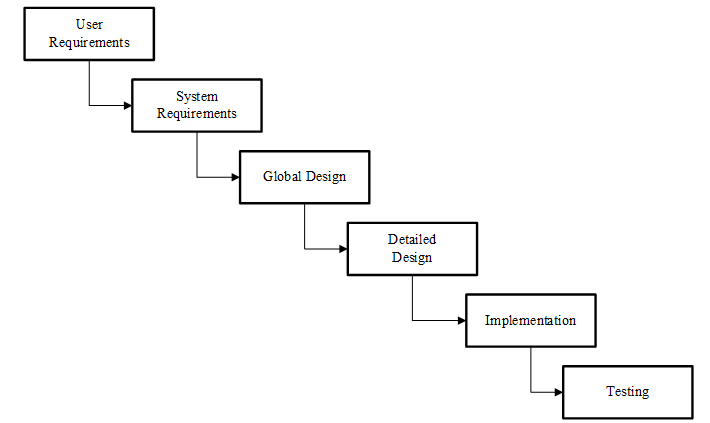
\includegraphics [height=8cm, width=13cm]{konten/gambar/gbr201.png}
	\caption{Metode Waterfall}
	\label{gbr201}
\end{figure}
%-----------------------------------------------------------------------------%
\section{Perancangan Sistem}
%-----------------------------------------------------------------------------%
Perancangan sistem adalah proses pembuatan rancangan suatu sistem berdasarkan hasil dari tahap analisis sistem. Dalam proses perancangan sistem memuat berbagai uraian mengenai input, proses, dan output dari sistem yang diusulkan (Setiawan, 2013).
Perancangan sistem bertujuan untuk memberikan gambaran apa yang seharusnya di kerjakan bagaimana tampilannya (Damayanti \& Sulistiani, 2017).
Perancangan sistem merupakan tahap selanjutnya setelah analisa sistem, mendapatkan gambaran dengan jelas tentang apa yang dikerjakan pada analisa sistem, maka dilanjutkan dengan memikirkan bagaimana membentuk sistem tersebut.Tujuan Perancangan Sistem (Kristanto, 2008):

\begin{enumerate}
	
	\item Untuk memenuhi kebutuhan pemakaian sistem (\textit{user}).
	\item Untuk memberikan gambaran yang jelas dan menghasilkan rancangan bangun yang lengkap kepada pemograman komputer dan ahli-ahli teknik lainnya yang terlibat dalam pengembangan atau pembuatan sistem
	
\end{enumerate}

%-----------------------------------------------------------------------------%
\section{Tahap Perancangan Sistem}
%-----------------------------------------------------------------------------%
Tahap perencanaan (\textit{planning}) adalah menyangkut studi tentang kebutuhan pengguna (\textit{user specification}), studi-studi kelayakan (\textit{feasibility study}) baik secara teknis maupun secara teknologi serta penjadwalan pengembangan suatu proyek sistem informasi atau perangkat lunak.

\subsection{ Analisis}
Langkah ini merupakan analisa terhadap kebutuhan sistem. Pengumpulan data dalam tahap ini bisa melakukan sebuah penelitian, wawancara atau studi literatur. Sistem analis akan menggali informasi sebanyak-banyaknya daripengguna (\textit{user}) sehingga akan tercipta sebuah sistem komputer yang bisa melakukan tugas-tugas yang diinginkan oleh pengguna (\textit{user}) tersebut. Tahapan ini akan menghasilkan dokumen (\textit{user requirtment} atau bisa dikatakan sebagai data yang berhubungan dengan keinginan (\textit{user} dalam pembuatan sistem. Dokumen ini lah yang akan menjadi acuan sistem analis untuk menerjemahkan ke dalam bahasa pemrogram.
\subsection{ Perancangan Interface}
Tahapan dimana dilakukan penuangan pikiran dan perancangan sistem terhadap solusi dari permasalahan yang ada dengan menggunakan perangkat pemodelan sistem seperti UML diantara seperti \textit{class diagram, use case diagram, activity diagram dan sequence diagram}.
\subsection{ Implementasi}
Tahap implementasi adalah adalah tahap dimana kita mengimplementasikan perancanagan sistem ke situasi nyata, disini kita akan berurusan dengan pemilihan perangkat keras dan penyusunan perangkat lunak.

\subsection{ Pengujian}
Tahap pengujian adalah tahap dimana sistem yang baru diuji kemampuan dan keefektifannya sehingga didapatkan kekurangan dan kelemahan sistem yang kemudian dilakukan pengkajian ulang dan perbaikan terhadap aplikasi menjadi lebih baik dan sempurna.
\subsection{ Pemeliharaan}
Perangkat lunak yang sudah disampaikan kepada pelanggan pasti akan mengalami perubahan. Perubahan tersebut bisa karena mengalami kesalahan karena perangkat lunak harus menyesuaikan dengan lingkungan baru, atau karena pelanggan membutuhkan perkembangan fungsional.
%-----------------------------------------------------------------------------%


%-----------------------------------------------------------------------------%
\section{Website}
%-----------------------------------------------------------------------------%
Menurut Kirana dalam Taufik (2017) menyatakan bahwa website atau situs merupakan tempat penyimpanan data dan informasi dengan menggunakan topik tertentu. Di umpamakan situs web ini adalah sebuah buku yang berisikan sebuah topik tertentu, website atau situs web juga merupakan kumpulan dari halaman- halaman web yang saling berkaitan di dalam web tersebut.
Menurut Anisya dan Yunita (2017) Web adalah sebuah penyebaran informasi melalui internet. Web merupakan hal yang tidak dapat di pisahkan dari dunia internet. Melalui web, setiap pemakai internet bisa mengakses informasi-informasi di situs web yang tidak hanya berupa teks, tetapi juga dapat berupa gambar, suara, film, animasi, dan lain-lain.
Secara umum ada beberapa bahasa pemograman yang di gunakan untuk membuat aplikasi website. Adapun bahasa program yang di pakai sebagai berikut:

\begin{enumerate}
	\item HTML \textit{ (Hyper Text Markup Language)}.
	\item PHP \textit{ (Pear Hypertext Preposessor)}.
	\item CSS \textit{ (Cascading Style Sheet)}.
	\item Javascript.
	\item Mysql.
	\item Jquery.

\end{enumerate}

\subsection{HTML}

HTML \textit{(Hyper Text Markup Language)} adalah sebuah bahasa markup yang digunakan untuk membuat halaman web dan menampilkan berbagai informasi di dalam sebuah browser internet (Anisya dan Yunita, 2017).
HTML \textit{(Hyper Text Markup Language)} merupakan bahsaa yang digunakan untuk mendeskripsikan struktur sebuah halaman web. HTML berfungsi untuk mempublikasikan dokumen online. Statement dasar dari HTML disebut tags. Sebuah tag dinyatakan dalam sebuah kurung siku. Tags yang ditujukan untuk sebuah dokumen atau bagian dari suatu dokumen haruslah dibuat berupa pasangan. Terdiri dari tag penutup menggunakan tambahan tanda garis miring (/) di awal nama tag.(Henderson dalam Omar dkk, 2018)

\subsection{Wampp}
%-----------------------------------------------------------------------------%
WAMPP merupakan salah satu paket \textit{installasi Apache, PHP dan MySQL}instant yang dapat kita gunakan untuk membantu proses installasi ketiga produk tersebut. Selain paket installasi instant WAMPP versi 3.2 juga memberikan fasiltias pilihan pengunaan PHP5 atau PHP7. Untuk berpindah versi PHP yang ingin digunakan juga sangat mudah dilakukan dengan mengunakan bantuan \textit{PHP Switch} yang telah disertakan oleh WAMP dan yang terpenting WAMP bersifat \textit{free} atau gratis untuk digunakan.
Sejarah singkat WAMP, WAMP merupakan pengembangan dari LAMP
\textit{(Linux Apache, MySQL, PHP and PERL)}, WAMP ini merupakan \textit{project} nonprofit yang di kembangkan oleh \textit{Apache Friends} yang didirikan Kai 'Oswalad'Seidler dan Kay Vogelgesang pada tahun 2002, \textit{project} mereka ini bertujuan mempromosikan pengunaan \textit{Apache} web server.

\subsection{PHP}
PHP \textit{(Pear Hypertext Preposessor)} merupakan sebuah bahasa Scripting yang di bundle dengan HTML yang di jalankan disisi \textit{Server}. Sebagian besar perintahnya berasal dari bahasa C, Java dan Perl dengan beberapa tambahan fungsi PHP (Anisya dan Yunita, 2017). Sedangkan, menurut Abdul dan Kasmawi (2016) PHP adalah salah satu skrip bahasa pemograman yang di rancang untuk membangun aplikasi \textit{web}. PHP dibangun dalam bentuk skrip yang di tempatkan dan di proses \textit{server}. Hasilnya akan dikirimkan ke \textit{client}, tempat pemakai menggunakan \textit{browser}. Secara khusus, PHP dirancang untuk membentuk web dinamis. Artinya, ia dapat membentuk suatu tampilan berdasarkan permintaan terkini, misalnya dapat menampilkan isi basis data ke halaman web.


\subsection{MySQL}
MySQL merupakan bahasa standar yang digunakan untuk memanipulasi data dan memperoleh data dari sebuah database relasional. SQL merupakan bahsa standar yang digunakan untuk memanipulasi data dan memperoleh data dari database relasional. SQL memungkinkan seorang pengguna untuk mengakses informasi tanpa mengetahui bagaimana informasi tersebut disusun. SQL dilengkapi dengan sejumlah perintah untuk melakukan manipulasi data. (Anisya dan Yunita, 2016)
MySQL adalah salah satu jenis \textit{database server} yang menggunakan SQL \textit{(Structured Query Language)} sebagai bahasa dasar untuk mengakses \textit{database-nya}. MySQL termasuk jenis \textit{Relational Database Management System}(RDBMS), sehingga istilah seperti tabel, baris dan kolom digunakan pada MySQL. MySQL sangat populer dikalangan pengembang perangkat lunak karena MySQL merupakan \textit{database server} yang gratis dan cepat. Selain itu, dukungan dari perusahaan dan komunitas yang memadai membuat MySQL menjadi \textit{database server} yang disukai dan termasuk dalam kategori database yang handal.(Arifudzaki dalam abdul dan kasmawi, 2016).

%-----------------------------------------------------------------------------%
\section{Dinas Kesehatan Kabupaten Pelalawan}
%-----------------------------------------------------------------------------%
\subsection{Visi dan Misi Instansi}

Mewujudkan Pelayanan Kesehatan Berkualitas dan Berkeadilan Menuju Masyarakat Pelalawan Sehat Untuk mencapai visi yang telah ditetapkan, maka ditetapkan misi Dinas Kesehatan sebagai berikut :
\begin{enumerate}
	
	\item Meningkatkan dan memantapkan manajemen dan kinerja serta pelayanan kesehatan yang terjangkau, bermutu, adil dan merata di semua tingkat administrasi dan unit-unit pelayanan kesehatan.
	
	\item Meingkatkan dan mengembangkan promosi kesehatan dan membudayakan Perilaku Hidup Bersih dan Sehat (PHBS) di masyarakat.
	
	\item Meningkatkan kinerja dan memperkuat 
	upaya-upaya pengendalian penyakit dan mewujudkan lingkungan
	sehat, serta penanggulan masalah gizi masyarakat.
	
	\item Meningkatkan kualitas Sistem Informasi Kesehatan (SIK).
	
	\item Memantapkan kemitraan lintas sektor dan pemberdayaan masyarakat.
\end{enumerate}

\subsection{Struktur Organisasi Instansi}
%-----------------------------------------------------------------------------%
Struktur organisasi pada dinas kesehatan kabupaten pelalawan dapat dilihat pada \pic~\ref{StrukturOrganisasi}

\begin{figure}
	\centering
	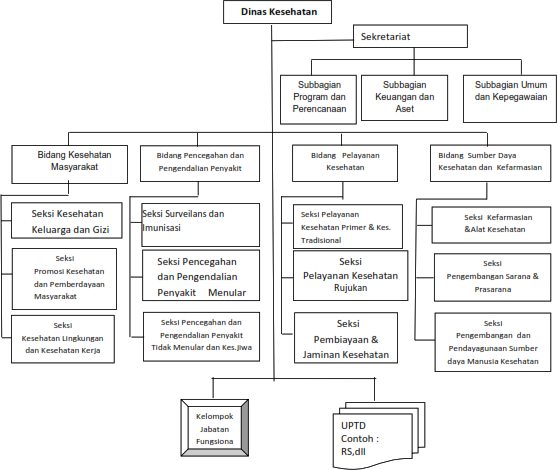
\includegraphics [height=13cm, width=13cm]{konten/gambar/StrukturOrganisasi.png}
	\caption{Struktur Organisasi}
	\label{StrukturOrganisasi}
\end{figure}

